\documentclass[12pt,twoside]{article}
%%%%%%%%%%%%%%%%%%%%%%%%%%%%%%%%%%%%%%%%%%%%%%%%%%%%%%%%%%%%%
% Meta informations:
\newcommand{\trauthor}{Ali Saleh}
\newcommand{\trtype}{Seminar Paper} %{Seminararbeit} %{Proseminararbeit}
\newcommand{\trcourse}{Neural Networks}
\newcommand{\trtitle}{Comparison of Gradient Descent Optimization Methods for Neural Networks}
\newcommand{\trmatrikelnummer}{6517831}
\newcommand{\tremail}{3saleh@informatik.uni-hamburg.de}
\newcommand{\trarbeitsbereich}{Knowledge Technology, WTM}
\newcommand{\trdate}{13.07.2017}

%%%%%%%%%%%%%%%%%%%%%%%%%%%%%%%%%%%%%%%%%%%%%%%%%%%%%%%%%%%%%
% Languages:

% Falls die Ausarbeitung in Deutsch erfolgt:
% \usepackage[german]{babel}
% \usepackage[T1]{fontenc}
% \usepackage[latin1]{inputenc}
% \usepackage[latin9]{inputenc}	 				
% \selectlanguage{german}

% If the thesis is written in English:
\usepackage[english]{babel} 						
\selectlanguage{english}

%%%%%%%%%%%%%%%%%%%%%%%%%%%%%%%%%%%%%%%%%%%%%%%%%%%%%%%%%%%%%
% Bind packages:
\usepackage{acronym}                    % Acronyms
\usepackage{algorithmic}								% Algorithms and Pseudocode
\usepackage{algorithm}									% Algorithms and Pseudocode
\usepackage{amsfonts}                   % AMS Math Packet (Fonts)
\usepackage{amsmath}                    % AMS Math Packet
\usepackage{amssymb}                    % Additional mathematical symbols
\usepackage{amsthm}
\usepackage{booktabs}                   % Nicer tables
\usepackage{float}
\usepackage{listings}
\usepackage{xcolor}
\usepackage{setspace}
\usepackage{appendix}

%\usepackage[font=small,labelfont=bf]{caption} % Numbered captions for figures
%\usepackage{color}                      % Enables defining of colors via \definecolor
\definecolor{uhhRed}{RGB}{254,0,0}		  % Official Uni Hamburg Red
\definecolor{uhhGrey}{RGB}{122,122,120} % Official Uni Hamburg Grey
\usepackage{fancybox}                   % Gleichungen einrahmen
\usepackage{fancyhdr}										% Packet for nicer headers
%\usepackage{fancyheadings}             % Nicer numbering of headlines

%\usepackage[outer=3.35cm]{geometry} 	  % Type area (size, margins...) !!!Release version
%\usepackage[outer=2.5cm]{geometry} 		% Type area (size, margins...) !!!Print version
%\usepackage{geometry} 									% Type area (size, margins...) !!!Proofread version
\usepackage[outer=3.15cm]{geometry} 	  % Type area (size, margins...) !!!Draft version
\geometry{a4paper,body={5.8in,9in}}

\usepackage{graphicx}                   % Inclusion of graphics
%\usepackage{latexsym}                  % Special symbols
\usepackage{longtable}									% Allow tables over several parges
\usepackage{listings}                   % Nicer source code listings
\usepackage{multicol}										% Content of a table over several columns
\usepackage{multirow}										% Content of a table over several rows
\usepackage{rotating}										% Alows to rotate text and objects
%\usepackage[hang]{subfigure}            % Allows to use multiple (partial) figures in a fig
%\usepackage[font=footnotesize,labelfont=rm]{subfig}	% Pictures in a floating environment
\usepackage{tabularx}										% Tables with fixed width but variable rows
\usepackage{url,xspace,boxedminipage}   % Accurate display of URLs
\usepackage{subcaption}

%%%%%%%%%%%%%%%%%%%%%%%%%%%%%%%%%%%%%%%%%%%%%%%%%%%%%%%%%%%%%
% Configurationen:

\hyphenation{whe-ther} 									% Manually use: "\-" in a word: Staats\-ver\-trag

%\lstloadlanguages{C}                   % Set the default language for listings
\DeclareGraphicsExtensions{.pdf,.svg,.jpg,.png,.eps} % first try pdf, then eps, png and jpg
\graphicspath{{./src/}} 								% Path to a folder where all pictures are located
\pagestyle{fancy} 											% Use nicer header and footer

% Redefine the environments for floating objects:
\setcounter{topnumber}{3}
\setcounter{bottomnumber}{2}
\setcounter{totalnumber}{4}
\renewcommand{\topfraction}{0.9} 			  %Standard: 0.7
\renewcommand{\bottomfraction}{0.5}		  %Standard: 0.3
\renewcommand{\textfraction}{0.1}		  	%Standard: 0.2
\renewcommand{\floatpagefraction}{0.8} 	%Standard: 0.5

% Tables with a nicer padding:
\renewcommand{\arraystretch}{1.2}

%%%%%%%%%%%%%%%%%%%%%%%%%%%%
% Additional 'theorem' and 'definition' blocks:
\theoremstyle{plain}
\newtheorem{theorem}{Theorem}[section]
%\newtheorem{theorem}{Satz}[section]		% Wenn in Deutsch geschrieben wird.
\newtheorem{axiom}{Axiom}[section] 	
%\newtheorem{axiom}{Fakt}[chapter]			% Wenn in Deutsch geschrieben wird.
%Usage:%\begin{axiom}[optional description]%Main part%\end{fakt}

\theoremstyle{definition}
\newtheorem{definition}{Definition}[section]

%Additional types of axioms:
\newtheorem{lemma}[axiom]{Lemma}
\newtheorem{observation}[axiom]{Observation}

%Additional types of definitions:
\theoremstyle{remark}
%\newtheorem{remark}[definition]{Bemerkung} % Wenn in Deutsch geschrieben wird.
\newtheorem{remark}[definition]{Remark} 

%%%%%%%%%%%%%%%%%%%%%%%%%%%%
% Provides TODOs within the margin:
\newcommand{\TODO}[1]{\marginpar{\emph{\small{{\bf TODO: } #1}}}}

%%%%%%%%%%%%%%%%%%%%%%%%%%%%
% Abbreviations and mathematical symbols
\newcommand{\modd}{\text{ mod }}
\newcommand{\RS}{\mathbb{R}}
\newcommand{\NS}{\mathbb{N}}
\newcommand{\ZS}{\mathbb{Z}}
\newcommand{\dnormal}{\mathit{N}}
\newcommand{\duniform}{\mathit{U}}

\newcommand{\erdos}{Erd\H{o}s}
\newcommand{\renyi}{-R\'{e}nyi}

%%%%%%%%%%%%%%%%%%%%%%%%%%%%%%%%%%%%%%%%%%%%%%%%%%%%%%%%%%%%
\lstdefinelanguage{custpython}{
    keywords={True, False, def, return, null, catch, switch, var, if, in, while, do, else, for},
    keywordstyle=\color{blue}\bfseries,
    ndkeywords={import, from, class},
    ndkeywordstyle=\color{mauve}\bfseries,
    identifierstyle=\color{black},
    sensitive=false,
    comment=[l]{\#},
    morecomment=[s]{/*}{*/},
    commentstyle=\color{gray}\ttfamily,
    stringstyle=\color{dkgreen}\ttfamily,
    morestring=[b]',
    morestring=[b]"
}

\lstdefinestyle{python}{
    language=custpython,
    backgroundcolor=\color{lightgray},
    extendedchars=true,
    basicstyle=\scriptsize\ttfamily,
    showstringspaces=false,
    showspaces=false,
    numbers=left,
    numberstyle=\ttfamily,
    numbersep=9pt,
    tabsize=2,
    breaklines=true,
    showtabs=false,
    captionpos=b,
    frame=shadowbox,
    rulesepcolor=\color{darkgray},
    belowcaptionskip=1\baselineskip,
    xleftmargin=1cm,
    xrightmargin=0.5cm,
    captionpos=b,
    literate={ö}{{\"o}}1
             {ä}{{\"o}}1
             {ü}{{\"o}}1
             {ß}{{\"ss}}1
}
%%%%%%%%%%%%%%%%%%%%%%%%%%%%%%%%%%%%%%%%%%%%%%%%%%%%%%%%%%%%%
% Document:
\begin{document}
\renewcommand{\headheight}{14.5pt}

\fancyhead{}
\fancyhead[LE]{ \slshape \trauthor}
\fancyhead[LO]{}
\fancyhead[RE]{}
\fancyhead[RO]{ \slshape \trtitle}

\lstdefinestyle{customc}{
  belowcaptionskip=1\baselineskip,
  breaklines=true,
  frame=L,
  xleftmargin=\parindent,
  language=C,
  showstringspaces=false,
  basicstyle=\footnotesize\ttfamily,
  keywordstyle=\bfseries\color{green!40!black},
  commentstyle=\itshape\color{purple!40!black},
  identifierstyle=\color{blue},
  stringstyle=\color{orange},
}

\lstdefinestyle{customasm}{
  belowcaptionskip=1\baselineskip,
  frame=L,
  xleftmargin=\parindent,
  language=[x86masm]Assembler,
  basicstyle=\footnotesize\ttfamily,
  commentstyle=\itshape\color{purple!40!black},
}

\lstset{escapechar=@,style=customc}

%%%%%%%%%%%%%%%%%%%%%%%%%%%%
% Cover Header:
\begin{titlepage}
	\begin{flushleft}
		Universit\"at Hamburg\\
		Department Informatik\\
		\trarbeitsbereich\\
	\end{flushleft}
	\vspace{3.5cm}
	\begin{center}
		\huge \trtitle\\
	\end{center}
	\vspace{3.5cm}
	\begin{center}
		\normalsize\trtype\\
		[0.2cm]
		\Large\trcourse\\
		[1.5cm]
		\Large \trauthor\\
		[0.2cm]
		\normalsize Matr.Nr. \trmatrikelnummer\\
		[0.2cm]
		\normalsize\tremail\\
		[1.5cm]
		\Large \trdate
	\end{center}
	\vfill
\end{titlepage}

	%backsite of cover sheet is empty!
\thispagestyle{empty}
\hspace{1cm}

%%%%%%%%%%%%%%%%%%%%%%%%%%%%
% Abstract:

% Abstract gives a brief summary of the main points of a paper:
\section*{Abstract}
Gradient Descent is the most widely used optimization method for neural networks training. This paper
aims to explore different algorithms for gradient optimization. Using standard datasets and different neural network architectures, time and complexity of the different algorithms will be compared and analyzed. 
% Lists:
\setcounter{tocdepth}{2} 					% depth of the table of contents (for Seminars 2 is recommented)
\tableofcontents
\pagenumbering{arabic}
\clearpage

%%%%%%%%%%%%%%%%%%%%%%%%%%%%
% Content:

% the actual content, usually separated over a number of sections
% each section is assigned a label, in order to be able to put a
% crossreference to it

\section{Introduction}
\label{sec:introduction}
In the scene of machine learning there are several key components to build a classification/regression model. Your model building usually involves several decision to make.
After choosing your model (e.g.KNN,  SVM, KART, NN, etc ...) you will begin to address the problem of how to choose your internal parameters (like the K in k nearest neighbor). For the
context of neural networks (assuming you have already chosen your model architecture) you will have to decide on how many layers, how many nodes per layer, what kind of encoding yo use, and several other parameters depending on your architecture. \cite{Schmidhuber201585} and \cite{Arel2010} have both presented the general outline for neural networks modeling in more details.
\bigskip

Once your model parameters are decided on you will need to begin the model training and evaluation. This is the process of deciding if your model is performing well, and can be used to compare several models together. In this setup evaluation is done by the mean of a loss function. It is used to asses the performance of you model by comparing predicted values against the ground truth of test data. Loss function is defined as :
\begin{equation}
  L(X, Y, \grave{Y})
\end{equation}

Where $X$ is your input, $Y$ is the ground truth, and $\grave{Y}$ is the prediction of your model on input.
\bigskip

In neural networks the output of your model depends highly on the weights of the connections between the network layers. This means that the notion of loss function is thus used to evaluate the goodness of a set of weights $W$ used by a model. Thus the need for optimization, to find the set of weights
that minimizes the loss function.
\bigskip

One of the most prominent strategies to optimize functions arises from calculus. From its name loss function is an ordinary mathematical function in the sense that it can have a derivative. Using the mathematical analogy, optimization can be achieved by moving in the direction of the gradient.
\bigskip

In a one variable function the first derivative is the rate of change of the function, which can be generalized into multi-variable functions. The gradient is the rate of change of a multi-variable function in a specified set of directions. It is represented as a vector of numbers, with each element of it as a rate of change in a direction. For a 3 variable function
\begin{equation}
  w=f(x,y,z)
\end{equation}
\\it is gradient in the 3 variables directions is :
\begin{equation}
 \nabla w = \bigg<  \frac{\partial w}{\partial x}, \frac{\partial w}{\partial y}, \frac{\partial w}{\partial z} \bigg>
\end{equation}

where $\frac{\partial w}{\partial x}$ is the partial derivative of the function w in the direction of x.
Moving the weights in the direction of the gradient leads to minimizing the loss function.

The reminder of this paper are organized as following. Section 2 will provide an overview of the gradient optimization methods, how to calculate them and what algorithms to compare. Section 3 will have a description of an experiment to compare the 3 algorithms together, section 4 will contain the results, section 5 will be a discussion, and Section 6 will conclude the paper.

\section{Gradient Computing And Optimization}
\label{sec:basics}
Computing the gradient for a function with hundreds of variables as in neural network is a computationally intensive function. Along the years tens of algorithms and approximations have been introduced to make it easier to compute the gradient of a function. In principle gradient can be computed in one of two ways. Either approximation using finite difference, or analytically using calculus.

In calculus the derivative of a single variable function is defined as :
\begin{equation}
  f'(x)=\lim_{h\to 0}\frac{f(x+h)-f(x)}{h}.
\end{equation}

Using finite difference to calculate the gradient you first specify step size (usually a tiny number to approximate $h$ approaching $0$). You then proceed to loop over all the variables in your function (here the weights) and you calculate the derivative for each one of them to obtain the gradient. Using the value obtained from this computation, the weights can be updated accordingly. The code snippet below describe a function to perform gradient using finite difference.

\lstinputlisting[language=Python]{Code/finite_diff.py}

The main problem with this way of computing the gradient is that it is computationally expensive. The loop over all the dimensions takes too much for a single step update. In a typical deep learning neural network the number of dimensions would be in the order of millions. Looping over millions of elements for a single update would result in weeks of network training. This is practically infeasible and thus comes the need to find another way for calculating the gradient of a function. 

A better way to compute the gradient for large number of dimensions is using closed formulas. To attain a closed formula you begin with your designated loss function at a single data point. You then differentiate it with respect to the weights to get your gradient formula \cite{Qian99onthe} \footnote{More information can be found here https://cs231n.github.io/optimization-1/}. It Is common to use sanity checks to compare the formula implementation results with the gradient computed using finite difference.

\subsection{Stochastic Gradient Descent}
Using the formula of gradient descent updating the parameters is a handy process. Use training set and weights evaluate your gradient and then update the weights according to the chosen learning rate. A sample python code to do this is below:
\lstinputlisting[language=Python]{Code/bgd.py}
this method is called batch gradient descent. All of the training data are used at once for training and evaluation of the gradient. It is guaranteed that batch gradient will always converge to the global minimum in convex optimization surface and to local minimum in non convex surfaces \cite{Ruder16}.

A more efficient way to compute the gradient is using smaller batches of the training data to evaluate the gradient. It is much faster and the shuffling of data used in this method enables to reaches new local minimums and not getting stuck with the first local minimum \cite{Ruder16}. Nevertheless slowly decreasing the learning rate would make the convergence of SGD similar to the batch gradient descent \cite{Ruder16}. A python snippet showing how to use this method is shown below:
\lstinputlisting[language=Python]{Code/bgd.py}
\subsection{Adagrad}
Adagrad is an optimization method that is using adaptive learning rates to compute the gradient \cite{Duchi2011}. Unlike SGD that has one learning rate for all the parameters, Adagrad has different learning rates that evolve over time with the parameters. For sparse datasets some parameters are more frequent than the others. Adagrad will have different learning rates for them the more frequent parameters will have a learning rate that decays faster and is smaller. The less frequent parameters on the other hand will have slower decaying learning rates that are larger.

Adagrad performs this by keeping track of a matrix all the past gradients for each parameter.While updating a parameter it divide the learning rate over the square roots of the sum all the gradients computed before for this parameter. Thus the more frequent a parameter the less the learning rate. One weakness of Adagrad is that over time the square roots of the sum becomes large that the learning rate become so small and no learning is happening after that

\subsection{Adam}
Adam (Adaptive Moment Estimation) is an adaptive learning optimizer like Adagrad \cite{Kingma2015}. Instead of keeping track of all the previous gradients to compute the squared sum as in Adagrad, Adam stores the average of all the past squares of the gradient along with another average of the past gradients themselves. The two averages works as an estimate of the first two moment (mean and variance). That is why the method is called this way.

In the original paper the two averages are initialized to zero which lead to them being biased toward zero, this led the authors to use a bias correction to resolve this problem. The two bias corrected averages are then used to update the parameters one by one. The update divide the learning rate by the bias-corrected average of the past squared gradients, and then multiply it by the  bias-corrected average of the past gradients. This lead to a less aggressive decaying of the learning rate for frequent parameters.

\section{Experiment Design}
\label{sec:model}
For comparing the algorithms mentioned in section 2, an experiment was held to analyze their performance.For the experiment the CIFAR10 dataset was used (see Figure \ref{cifar10}.  "The CIFAR-10 dataset consists of 60000 32x32 colour images in 10 classes, with 6000 images per class. There are 50000 training images and 10000 test images." \cite{Krizhevsky2009}. 

The model architecture used is convolution neural network. The model consists of the following layers. The first layer is a convolution layer with 32 filter each on 3 x 3 sub-regions with ReLU activation function. Then there are a max-pooling layer with 2 x 2 filters and a stride of 2 (to specify the factor by which to downscale), and dropout regularization rate of $0.25$  \cite{srivastava14a}. The next layer is a convolution layer with 64 filter each on 3 x 3 sub-region again with relu activation layer. Followed by another max-pooling layer with the same specifications as before. A flattening layer is then added which takes the 2D output of the previous layer and turn it into 1D (e.g. a 32 x 32 matrix would be 1024 array). After that comes a fully connected (dense) layer with ReLU activation and dropout regularization rate of $.5$. The final layer is another dense layer with size set to the number of classes (here 10) with softmax activation function. This layer with softmax outputs a probability of an image belonging to each class.

The model is then used with the 3 chosen optimizers. Each run consists of loading the cifar10 data set into two parts. The training set which consists of 50000 $32 x 32$ images. the testing set which consists of 10000 $32 x 32$ images. The training is then carried with batches of size 32. The training is done over 200 epochs. Categorical cross-entropy is used as loss function \cite{Boer2007}

\begin{figure}[H]
\centering
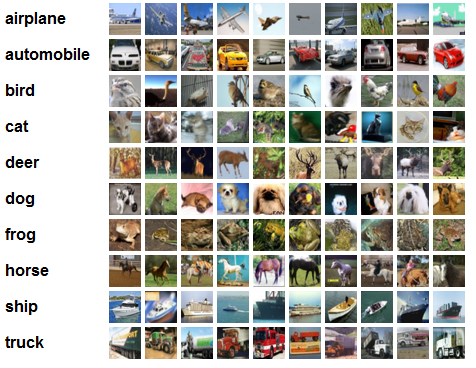
\includegraphics[scale=.8]{Code/cifar_preview.png}
\caption{overview of the CIFAR 10 dataset (courtesy of Alex Krizhevsky)}
\label{cifar10}
\end{figure}

The 5 metrics that were used for the comparison are:
\begin{itemize}
\item The total time an epoch takes to finish.
\item The final loss on the test set.
\item The accuracy of classification on the test set.
\item The final loss on the validation set.
\item The accuracy of classification on validation set.
\end{itemize}

The network parameters were initially set to the defaults provided by keras. A trial for optimization using hyperas (Keras + Hyperopt python library) was undergoing. Due to the sheer amount of parameters it is data was not considered for the analysis and the results with default parameters were used instead. Nevertheless the code for the optimization is provided in appendix B.


\section{Results}
\label{sec:results}

The execution time was measure by keras library for each epoch. As seen in Figure \ref{fig:time} the time for each epoch is not decaying over time. While the Adagrad has almost uniform time for each epoch, the SGD time fluctuates a lot, and the ADAM time is a reverse of SGD . At the beginning the SGD time was higher the the other two. Over time SGD began to stabilize with a spike around every 50 epoch. In the same time ADAM that began with smooth uniform time per epoch suddenly began to fluctuate randomly.

\begin{figure}[H]
\label{time}
\centering
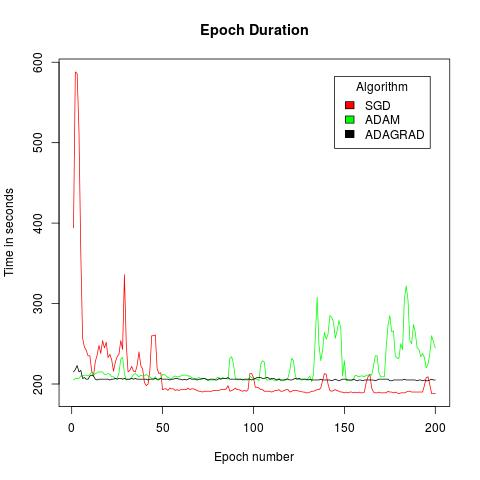
\includegraphics[scale=.7]{Code/Time.jpg}
\caption{Total execution time per epoch over time for each optimizer}
\label{fig:time}
\end{figure}

The loss of each of the 3 optimizers over epochs is shown in figures \ref{fig:loss} and \ref{fig:loss_val} for test and validation respectively. The two figures looks similar in shape. In both of them SGD begins with the highest loss and proceeds to reach the lowest loss of all of them. Both Adagrad and Adam begins at comparable loss values, but Adam's loss curve is less steep over time. In the end Adagrad reaches a lower loss value than Adam for both testing and validation. As expected the validation loss values are more fluctuating than the testing loss values, although Adam has considerably higher fluctuation  than the rest of the optimizers
\begin{figure}[H]
  \centering
  \begin{subfigure}{.5\textwidth}
    \centering
    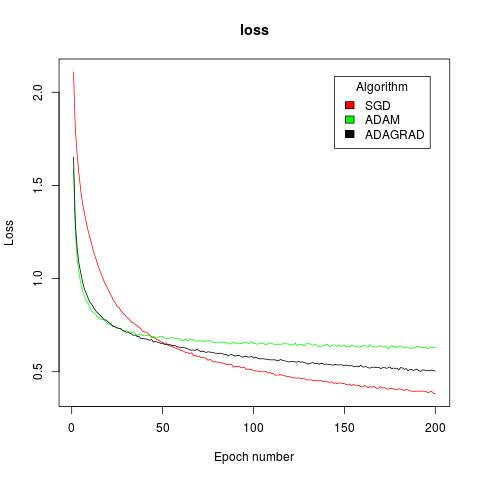
\includegraphics[scale=.46]{Code/loss.jpg}
    \caption{Loss per epoch on test set}
    \label{fig:loss}
  \end{subfigure}%
  \begin{subfigure}{.5\textwidth}
    \centering
    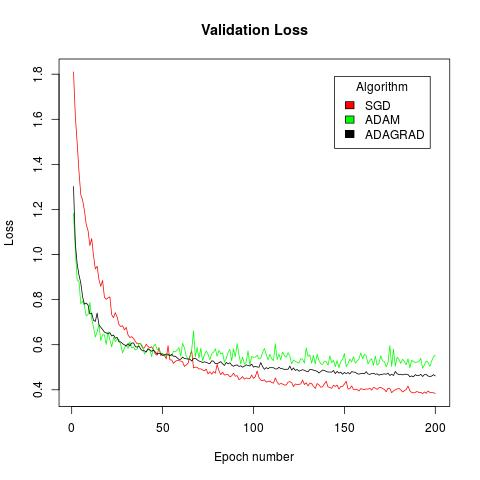
\includegraphics[scale=.46]{Code/val_loss.jpg}
    \caption{Loss per epoch for on validation set}
    \label{fig:loss_val}
  \end{subfigure}%
\end{figure}

\begin{figure}[H]
  \centering
  \begin{subfigure}{.5\textwidth}
    \centering
    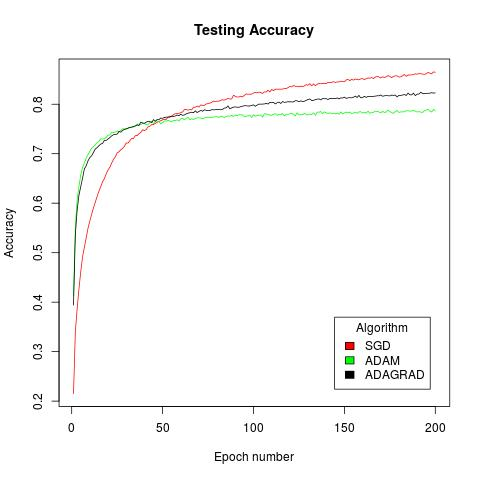
\includegraphics[scale=.45]{Code/acc.jpg}
    \caption{Accuracy on test set}
    \label{fig:acc}
  \end{subfigure}%
  \begin{subfigure}{.5\textwidth}
    \centering
    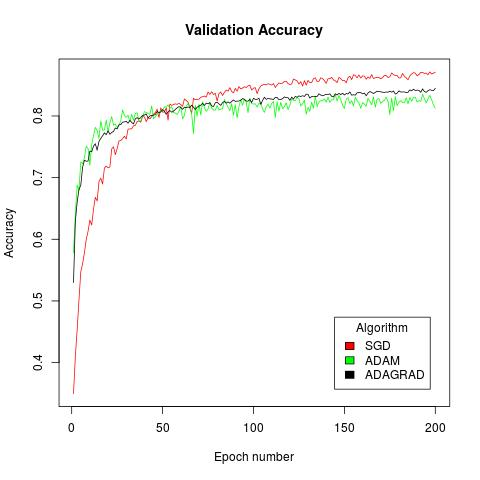
\includegraphics[scale=.45]{Code/val_acc.jpg}
    \caption{Accuracy on validation set}
    \label{fig:acc_val}
  \end{subfigure}%
\end{figure}

The same can be seen in the results of the accuracy. The accuracy of each of the 3 optimizers over epochs is shown in figures \ref{fig:acc} and \ref{fig:acc_val} for test and validation respectively. Again SGD has the highest accuracy although it began with the lowest both on testing and validation.  The same is still true for Adam and Adagrad, both begin similarly and end with Adgrad has higher accuracy than Adam. The validation accuracy fluctuation is still more prominent on Adam than the other two.

\section{Discussion}
The results show in section \ref{sec:results} along with the statistics show in table \ref{tab:hresult}, shows that on this dataset SGD outperform better than the other two optimizers. The design of the Adam and Adagrad is concerned much about the sparsity and in-frequent parameters. Much of the tweaking done in the two optimizers is targeting this point. With a balanced dense dataset like the CIFAR10 it's not a surprise that those two aren't performing well compared to the SGD. This is matching the state-of-art results on the CIFAR10 \cite{Graham14} \cite{Graham14a} \cite{SpringenbergDBR14} \cite{MishkinM15}. Although some of them are also using momentum (\cite{Qian99onthe}) component with SGD.

\begin{table}[H]
\caption{Experiment Statistics} %title of the table
\centering % centering table
\begin{tabular}{c r|r|r|r|r|r|r|r|r} % creating eight columns
\hline\hline %inserting double-line
\multicolumn{1}{c}{} &\multicolumn{3}{c}{SGD} &\multicolumn{3}{c}{Adam} &\multicolumn{3}{c}{Adagrad}\\ [0.5ex]
Metric & \textbf{min}& \textbf{mean} &\textbf{max} & \textbf{min}& \textbf{mean} &\textbf{max} & \textbf{min}& \textbf{mean} &\textbf{max}\\
\hline % inserts single-line
Time(seconds) & 188.0& 209.2 & 588.0& 203.0& 220.6& 322.0& 205.0& 206.1& 223.0 \\ % Entering row contents
\hline
Loss  & 0.3822 & 0.6041 & 2.1094& 0.6224& 0.6836& 1.5892& 0.5027& 0.6187& 1.6527 \\
\hline
Accuracy & 0.2151 & 0.7865 & 0.8654& 0.4132& 0.7655& 0.7899& 0.3942& 0.7827& 0.8242 \\[1ex] % [1ex] adds vertical space
\hline
Validation Loss  & 0.3828 & 0.5363 & 1.8103& 0.4953& 0.5708& 1.1835& 0.4577& 0.5391& 1.3018 \\
\hline
Validation Loss & 0.3496 & 0.8150 & 0.8715& 0.5782& 0.8075& 0.8353& 0.5298& 0.8131& 0.8449 \\[1ex] % [1ex] adds vertical space
\hline % inserts single-line
\end{tabular}
\label{tab:hresult}
\end{table}

The performance of Adam on validation sets is notable with it's high fluctuations. This can be attributed to the adaptive learning rates used in Adam. With a dense dataset, the work Adam do to maintain adaptive learning rate for each of the parameters doesn't seem to contribute much to its performance. It was always keeping track of the much information on the gradient of previous runs, this could be the reason it was fluctuating in performance over different unseen validation sets. 

All of that said, it's worth mentioning that SGD is not an all around solution. SGD takes time and in total it took more time to finish than the other two. Also it took around 50 epochs to stabilize in time and performance. It also took around 50 epochs to surpass the other two. With the small CIFAR10 it was plausible to train an SGD model in around 13 hours in a personal machine. The other two algorithms took around 1 hour less with the same hardware and configurations.

\section{Conclusion}
\label{sec:concl}
Choosing an optimization method for a model is not working according to a check list. There are hundreds of factors to consider. How to choose the parameters for the method is also a factor. If your data is sparse then an adaptive learning method (Adam/Adagrad)  would have an advantage. You can always begin with a simple SGD optimizer and build upon it but adding momentum then maybe converting to a more advanced adaptive learning method if needed.

%%%%%%%%%%%%%%%%%%%%%%%%%%%%%%%%%%%%%%
% hier werden - zum Ende des Textes - die bibliographischen Referenzen
% eingebunden
%
% Insbesondere stehen die eigentlichen Informationen in der Datei
% ``bib.bib''
%

\bibliographystyle{apalike}
\addcontentsline{toc}{section}{Bibliography}% Add to the TOC
\bibliography{bib}
\newpage

\begin{appendices}
\section{Appendix A}
The code used for the optimizers  evaluation:
\lstinputlisting[language=Python]{Code/cifar10.py}

\section{Appendix B}
The code used for hyper-parameter optimization:
\lstinputlisting[language=Python]{Code/cifar10_hyperas.py}
\end{appendices}
\end{document}
